\chapter{Perceptual Experiments}
\label{chap:PerceptualExperiments}

\section{Reconstruction of Individual Harmonics}
\label{sec:PerceptualExperiments-Reconstruction}
	An experiment was conducted to evaluate which harmonic excitation method is best suited to the generation of
	individual harmonics. A primary aim of this experiment was to determine whether any of the methods would cause a
	tone from a single instrument to be perceived as coming from multiple sources. Each method was used to reconstruct
	signals which from which some harmonic content had been removed. The quality of the reconstruction was assessed by
	participants in a multiple stimulus listening test. 

	\note{The same stimuli from chapter 6 are used.}

	For each stimuli the third through ninth harmonics were removed. Spectrograms of the cello stimulus before and after
	this process are shown in Figures \ref{fig:CelloSpectrogram} and \ref{fig:CelloFilteredSpectrogram}.  Test stimuli
	were then created by reintroducing these harmonics using SSBA, IAP and a synthesis method.  The synthesis method
	consisted of using the STFT to measure the amplitude envelope of the fundamental frequency and applying this to a
	synthesised sine wave at the frequency of the desired harmonic. 

	\begin{figure}[h!]
		\centering
		\captionsetup[subfigure]{oneside,margin={1cm, 0cm}}
		\subfloat[Unprocessed Stimulus]
		{
			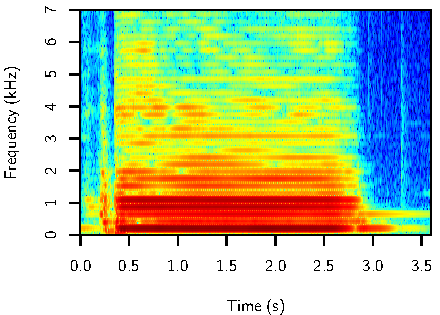
\includegraphics{chapter7/Images/CelloSpectrogram.pdf}
			\label{fig:CelloSpectrogram}
		}
		\quad
		\subfloat[Filtered Stimulus]
		{
			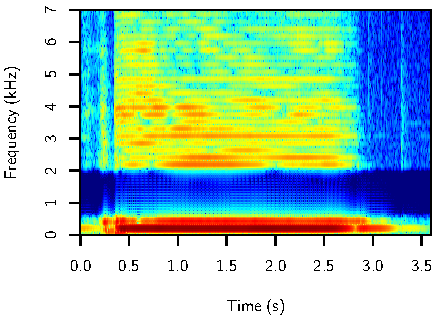
\includegraphics{chapter7/Images/CelloFilteredSpectrogram.pdf}
			\label{fig:CelloFilteredSpectrogram}
		}
		\caption{Spectrograms of the cello stimulus.}
		\label{fig:CelloSpectrograms}
	\end{figure}

	Each stimulus was reconstructed three times using each method, using different parameters each time. For the SSBA
	and IAP methods a different order FIR filter was used to isolate the fundamental frequency. The filters used had
	orders of 50, 100 and 500. For the synthesis method the window length of the STFT was changed, taking values of 50,
	100 and 500 samples. Spectrograms for the reconstructed stimuli, using the smallest filter order / STFT window
	length, are shown in Figure \ref{fig:ReconstructedCelloSpectrograms}.

	\begin{figure}[h!]
		\centering
		\captionsetup[subfigure]{oneside,margin={1cm, 0cm}}
		\subfloat[SSBA with a 50\super{th} order filter.]
		{
			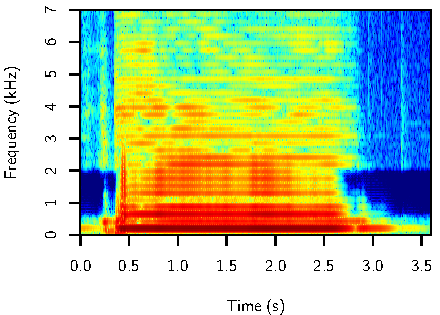
\includegraphics{chapter7/Images/CelloSSBASpectrogram.pdf}
			\label{fig:CelloSSBASpectrogram}
		}
		\quad
		\subfloat[IAP with a 50\super{th} order filter.]
		{
			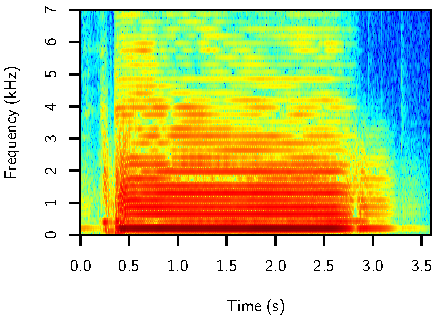
\includegraphics{chapter7/Images/CelloIAPSpectrogram.pdf}
			\label{fig:CelloIAPSpectrogram}
		}
		
		\subfloat[Synthesis with an STFT window length of 50 samples.]
		{
			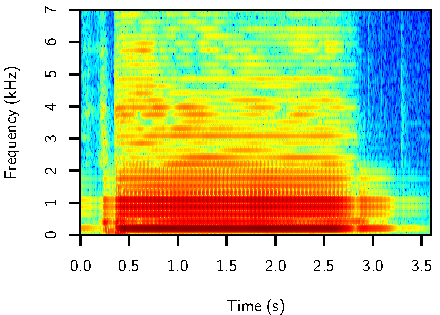
\includegraphics{chapter7/Images/CelloSynthesisSpectrogram.pdf}
			\label{fig:CelloSynthesisSpectrogram}
		}
		\caption{Spectrograms of the cello stimulus reconstructed using three different methods.}
		\label{fig:ReconstructedCelloSpectrograms}
	\end{figure}

	On inspection of these spectrograms the characteristics of the three excitation methods can be seen. The amplitude
	envelopes of the generated harmonics differ greatly between the methods. Comparing the decay portion of the
	envelopes compared with those in the original signal (Figure \ref{fig:CelloSpectrogram}) highlights these
	differences. In the cello stimulus the fundamental frequency and third harmonic have a longer decay time then the
	other harmonics. The harmonics generated by the IAP and synthesis methods (Figures \ref{fig:CelloIAPSpectrogram} and
	\ref{fig:CelloSynthesisSpectrogram}) use the amplitude envelope of the fundamental frequency extending the decay
	time of the these harmonics compared to that in the original. Those generated by the SSBA method (Figure
	\ref{fig:CelloSSBASpectrogram}) have shortened decay times. As the order of the harmonic is increased the decay time
	gets shorter due to the dynamic expansion shown in Figure \ref{fig:SSBATemporalEffects}.

	The amplitude envelopes of the harmonics generated using the synthesis techniques exhibit a large amount of ripple.
	This is due to the amplitude of the fundamental being calculated in blocks. These inaccuracies are not present in
	the harmonics generated using the IAP method as the amplitude is calculated on a sample by sample basis.

	Test participants were presented with all processed version of a particular stimulus at once along with a reference
	stimulus (the unprocessed stimulus) and an anchor stimulus (the stimulus with its harmonics removed).  Participants
	were asked to grade how well each processed stimulus recreated the reference stimulus on a scale from 0 to 100.

	The results of this experiment are shown in Figure \ref{fig:SMCResults} with error bars showing the 95\% confidence
	intervals. The stimuli numbers refer to different processing algorithms as follows.

	\begin{tabular}{>{\bfseries}rl}
		1. & The reference stimulus. \tabularnewline
		2. & Stimulus reconstructed using the synthesis method with an STFT window length of 50
		     samples. \tabularnewline
		3. & Stimulus reconstructed using the synthesis method with an STFT window length of 100
		     samples. \tabularnewline
		4. & Stimulus reconstructed using the synthesis method with an STFT window length of 500
		     samples. \tabularnewline
		5. & Stimulus reconstructed using the SSBA method using a 50\super{th} order filter. \tabularnewline
		6. & Stimulus reconstructed using the SSBA method using a 100\super{th} order filter. \tabularnewline
		7. & Stimulus reconstructed using the SSBA method using a 500\super{th} order filter. \tabularnewline
		8. & Stimulus reconstructed using the IAP method using a 50\super{th} order filter. \tabularnewline
		9. & Stimulus reconstructed using the IAP method using a 100\super{th} order filter. \tabularnewline
		10. & Stimulus reconstructed using the IAP method using a 500\super{th} order filter. \tabularnewline
		11. & Stimulus with third through ninth harmonics removed (anchor).
	\end{tabular}

	\begin{figure}[h!]
		\centering
		\captionsetup[subfigure]{oneside,margin={1cm, 0cm}}
		\subfloat[Cello Stumulus]
		{
			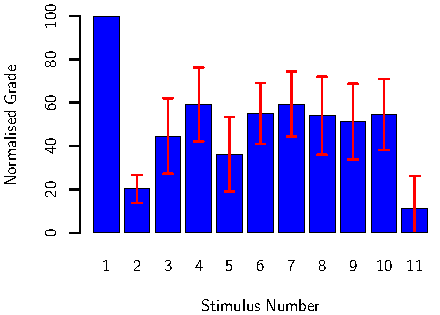
\includegraphics{chapter7/Images/CelloResults.pdf}
			\label{fig:CelloResults}
		}
		\quad
		\subfloat[Clarinet Stimulus]
		{
			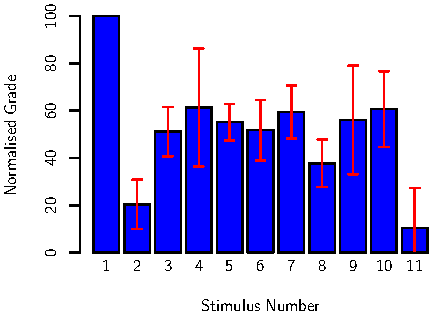
\includegraphics{chapter7/Images/ClarinetResults.pdf}
			\label{fig:ClarinetResults}
		}

		\subfloat[Synthesised Stimulus]
		{
			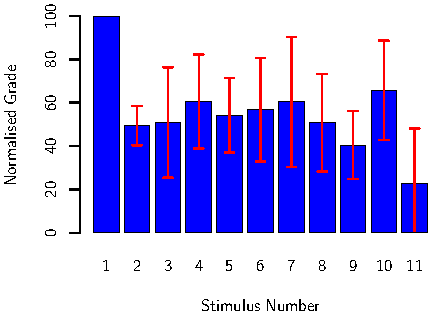
\includegraphics{chapter7/Images/SynthResults.pdf}
			\label{fig:SynthResults}
		}
		\quad
		\subfloat[Piano Stimulus]
		{
			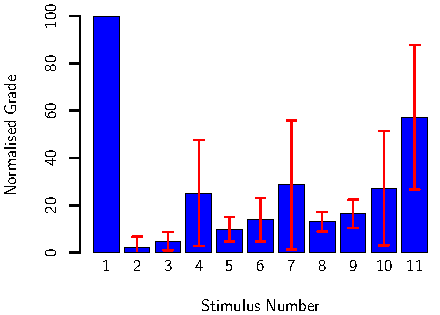
\includegraphics{chapter7/Images/PianoResults.pdf}
			\label{fig:PianoResults}
		}
		\caption{Mean grades and confidence intervals for each of the stimuli.}
		\label{fig:SMCResults}
	\end{figure}

	Across all the stimuli there is a general increase in the perceived quality of the reproduction as the filter order
	or STFT window length is increased. With the SSBA and IAP methods increasing the filter order increases the level
	difference between the fundamental and its harmonics, better isolating the fundamental.  This is turn reduces the
	levels of intermodulation distortion in the output producing a `cleaner' harmonic.  With the synthesis method
	increasing the STFT window length increases the frequency resolution allowing for the amplitude envelope of the
	fundamental frequency to be measured more precisely.

	The piano stimulus used had very little energy at its fundamental frequency. This illustrates the problem discussed
	previously, there is not enough information in the amplitude envelope of the fundamental to reproduce the other
	harmonics. This leads to much lower grades for the reproduced signals than for any of the other stimuli. Figure
	\ref{fig:PianoResults} shows that the piano stimulus with its harmonics missing received a higher grade on average
	then any of the reconstructed stimuli further showing how poor the quality of the reconstructions is.

	The confidence intervals for the grades given to the majority of the stimuli are high. This is most likely due to
	there being too few participants in the experiment. To supplement these results each of the stimuli was graded with
	the R\sub{nonlin} metric. These results were normalised to the same range as the results from the listening test and
	are displayed in Figure \ref{fig:SMCRNonlin}.

	\begin{figure}[h!]
		\centering
		\captionsetup[subfigure]{oneside,margin={1cm, 0cm}}
		\subfloat[Cello Stimulus]
		{
			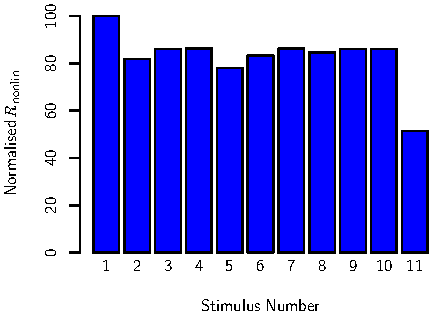
\includegraphics{chapter7/Images/CelloRNonlin.pdf}
			\label{fig:CelloRNonlin}
		}
		\quad
		\subfloat[Clarinet Stimulus]
		{
			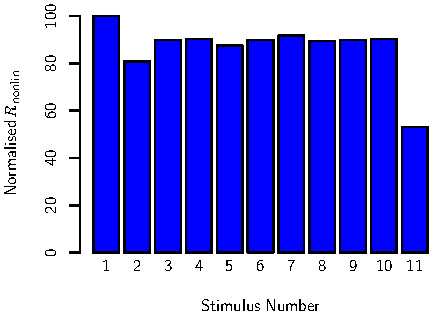
\includegraphics{chapter7/Images/ClarinetRNonlin.pdf}
			\label{fig:ClarinetRNonlin}
		}

		\subfloat[Synthesised Stimulus]
		{
			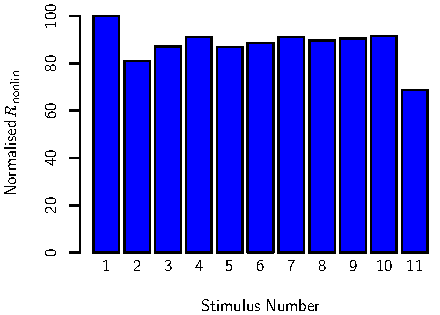
\includegraphics{chapter7/Images/SynthRNonlin.pdf}
			\label{fig:SynthRNonlin}
		}
		\quad
		\subfloat[Piano Stimulus]
		{
			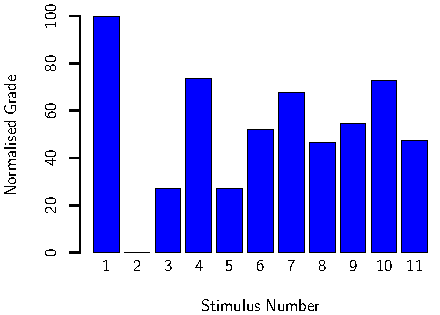
\includegraphics{chapter7/Images/PianoRNonlin.pdf}
			\label{fig:PianoRNonlin}
		}
		\caption{R\sub{nonlin} values for each of the stimuli.}
		\label{fig:SMCRNonlin}
	\end{figure}

	The R\sub{nonlin} values support the correlations found in the listening test results. Using a higher order filter
	to isolate the fundamental improves the quality of the reconstruction. Figure \ref{fig:PianoRNonlin} again
	illustrates the problems which arise when the input signal has little energy at its fundamental frequency. Several
	of the reconstructions are objectively less similar to the original stimulus than the anchor stimulus is.

	Both sets of results show that, using the highest order filter / STFT window lengths, each of the methods produce
	similar quality reconstructions of the original signal. For shorter filter lengths the IAP method provides more
	quality at then the SSBA method at the expense of requiring slightly more computation. The synthesis method produces
	similar quality results but incurs further computational complexity. 

	For timbral control applications the IAP method provides the greatest flexibility. For the majority of stimuli in
	this experiment it reproduced signals with the highest perceived quality. It was also shown in section
	\ref{sec:ExcitationEvaluation-Comparison-Homogeneity} that it is a homogeneous process allowing it to be applied to
	a wider range of signals with more predictable effects.

\section{Semantic Control}
\label{sec:PerceptualExperiments-SemanticControl}
	The findings of Chapter \ref{chap:TimbreEvaluation} can be combined with the techniques discussed in Chapter
	\ref{chap:FeatureControl} to develop audio effects with control parameters which relate to specific descriptive
	terms. In this section two such effects are developed and their performance evaluated. Each of these effects have a
	single `semantic' control parameter which changes processing parameters based three related semantic terms. The
	first effect, the warmth / harshness effect, is intended to introduce `warmth' for low values of the
	control parameter, `brightness' for middle values of the control parameter and `harshness' for high values of the
	control parameter. The second effect, the harshness / crunchiness effect, is intended to change between
	`harshness', `brightness' and `crunchiness' for different values of the control parameter.

	The performance of each effect is evaluated using a set of ten test signals, comprising two electric bass guitars
	(B1 and B2), a flute (F), two electric guitars (G1 and G2), a marimba (M), an oboe (O), a saxophone (S), a trumpet
	(T) and a violin (V). The signals were adjusted to have equal loudness prior to experimentation.  Firstly the
	effects are evaluated objectively by comparing them to the analysis performed in Chapter
	\ref{chap:TimbreEvaluation}. Secondly the effects are evaluated subjectively as discussed in Sections
	\ref{sec:PerceptualExperiments-SemanticControl-EvaluationExperiment} and
	\ref{sec:PerceptualExperiments-SemanticControl-PerformanceResults}.

	\subsection{Semantically Controlled Effect Design}
	\label{sec:PerceptualExperiments-SemanticControl-EffectDesign}
		This section describes the underlying systems of the warmth / harshness and harshness / crunchiness effects
		and the operation of their control parameters. The performance of each effect is evaluated objectively by
		examining how they manipulate the features of the test signals. Each effect is used to process each of the
		test signals with its parameter set to the minimum value, the middle value and the maximum value,
		corresponding to `warm', `bright' and `harsh' for the warmth / harshness effect and `harsh', `bright' and
		`crunchy' for the harshness / crunchiness effect. The audio features of the unprocessed and processed
		signals in each of these applications are calculated in the same manner as in the SAFE plug-ins. These audio
		features are the compared to those taken from the SAFE dataset.

		As discussed in Chapter \ref{chap:TimbreEvaluation} the terms `warm', `harsh' and `bright' are all used to
		describe transformations applied by both distortion and equalisation effects. `Harsh' and `bright' having
		different definitions depending on the type of processing applied. The objective performance of the effects
		proposed in this section is evaluated against data from both the SAFE distortion and equaliser. In order to
		do this, two new timbre spaces are constructed by performing PCA on the processed audio features and feature
		differences of the combined distortion and equaliser data. Two performance scores are given to each
		combination of audio effect, descriptor and test signal. The first measuring how close the processed
		features of the signal are to points labelled with the descriptor in the processed feature timbre space.
		The second measuring how close the changes in features caused by the effect are to points labelled with the
		descriptor in the feature difference timbre space.

		The performance of a particular effect, with a particular parameter setting on a particular test signal is
		measured by projecting the extracted audio features to a point on the relevant timbre space. The processed
		features of the signal are projected onto the processed feature timbre space and the feature differences
		onto the feature difference timbre space. The Mahalanobis distance, $M(x, d)$, between this point, $x$, and
		the distribution of transforms labelled with the descriptor, $d$, is taken using Equation
		\ref{eq:Mahalanobis}
		
		\begin{equation}
			M(x, d) = \sqrt{(x - \mu_{d})^{T}\Sigma_{d}^{-1}(x - \mu_{d})}
			\label{eq:Mahalanobis}
		\end{equation}

		Where $x$ is a column vector containing the coordinates of the point in the timbre space, $\mu_{d}$ a column
		vector containing the mean coordinates of all transforms in the timbre space labelled with descriptor $d$
		and $\Sigma_{d}$ the covariance matrix of those transforms' coordinates in the timbre space. The number of
		coordinates used in the calculation of Mahalanobis distance is determined in the same manner as discussed in
		Section \ref{sec:TimbreEvaluation-Analysis-Agreement}. Where there more than five transforms in the
		distribution, the coordinates in the first five PCs of the timbre space are used. Where the number of points
		in the distribution, $N_{d}$, is lower, only the first $N_{d} - 1$ coordinates can be used in order to avoid
		$\Sigma_{d}$ being singular.

		Where the descriptor, $d$, is represented by two distributions of transforms, one from the distortion and
		one from the equaliser, the Mahalanobis distance from both distributions is taken and the minimum distance
		kept as the measure of performance.

		\subsubsection*{Warmth / Harshness}
			The warmth / harshness effect controls the spectral centroid of a signal using a refined version of
			the system given in Figure \ref{fig:TwoBandSpectralCentroidSystem}. Two spectral bands are
			generated, one with a spectral centroid lower than the input signal and one with a higher spectral
			centroid than the input signal. The relative levels of these bands is then adjusted in order to
			adjust the output's spectral centroid. The full system is shown in Figure \ref{fig:WarmHarsh}.

			\begin{figure}[h!]
				\centering
				\begin{tikzpicture}
					\node (In) at (-1, -3.25) {$x[n]$};
					\coordinate (InMid) at (0, -3.25);
					\draw (In) -- (InMid);

					\coordinate (Side1) at (0, -1.25);
					\coordinate (Side2) at (0, -2.25);
					\draw (InMid) -- (Side2);
					\draw (Side2) -- (Side1);

					\node (F0) [draw] at (2, -1.25) {$f_{0}$ Tracker};
					\node (F0Filter) [draw] at (2, -2.25) {LPF};
					\draw (Side2) -- (F0Filter);
					\draw (F0) -- (F0Filter);
					\draw (Side1) -- (F0);

					\node (Centroid) [draw] at (2, -3.25) {$\mu_{s}$ Tracker};
					\draw (InMid) -- (Centroid);

					\node (Add) [operator] at (9.75, -3.25) {+};

					% NLD
					\node (NLD) [draw] at (4.5, -2.25) {Nonlinear Device};
					\draw (F0Filter) -- (NLD);

					\node (NLDFilter) [draw] at (7, -2.25) {HPF};
					\draw (NLD) -- (NLDFilter);

					\node (NLDGain) [gain] at (8.25, -2.25) {};
					\draw (NLDFilter) -- (NLDGain);
					\coordinate (NLDOut) at (8.75, -2.25);
					\draw (NLDGain) -- (NLDOut);
					\draw (NLDOut) -- (Add);

					\coordinate (NLDSide) at (7, -3.25);
					\draw (Centroid) -- (NLDSide);
					\draw (NLDSide) -- (NLDFilter);

					% through
					\coordinate (Through) at (0, -4.25);
					\node (ThroughFilter) [draw] at (2, -4.25) {LPF};
					\draw (Through) -- (ThroughFilter);
					\draw (Side2) -- (Through);
					\draw (Centroid) -- (ThroughFilter);
					\node (ThroughGain) [gain] at (8.25, -4.25) {};
					\coordinate (ThroughOut) at (8.75, -4.25);
					\draw (ThroughFilter) -- (ThroughGain);
					\draw (ThroughGain) -- (ThroughOut);
					\draw (ThroughOut) -- (Add);

					\node (Out) at (11, -3.25) {$y[n]$};
					\draw (Add) -- (Out);
				\end{tikzpicture}
				\caption{The system employed in the warmth / harshness effect.}
				\label{fig:WarmHarsh}
			\end{figure}

			The low frequency band is generated by low pass filtering the input signal at its spectral centroid.
			The high frequency band is generated by applying a static nonlinearity to the isolated $f_0$ of the
			input signal and high pass filtering at the input's spectral centroid. Separating the bands at the
			spectral centroid in this way ensures that their respective spectral centroids sit either side of
			the input's.

			\begin{figure}[h!]
				\centering
				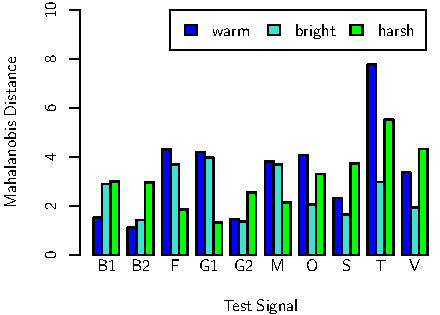
\includegraphics{chapter7/Images/HarshProcessedJeffsDistance.pdf}
				\caption{Mahalanobis distances for the processed 
					 features of the warmth / harshness effect.}
				\label{tab:HarshProcJeff}
			\end{figure}

			\begin{figure}[h!]
				\centering
				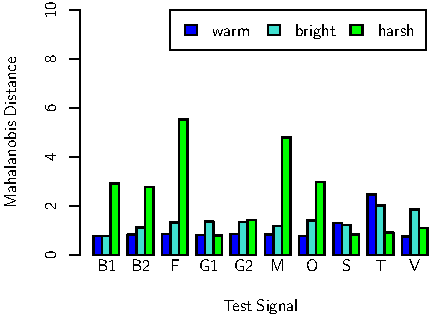
\includegraphics{chapter7/Images/HarshDifferenceJeffsDistance.pdf}
				\caption{Mahalanobis distances for the feature differences of 
					 the warmth / harshness effect.}
				\label{tab:HarshDiffJeff}
			\end{figure}

		\subsubsection*{Harshness / Crunchiness}
			\note
			{
				Based on the techniques discussed in Section
				\ref{sec:FeatureControl-Parameterisation-Irregularity}. Only 6 harmonics controlled and a
				surrogate harmonic profile is used to ease computational load.
			}

			\begin{figure}[h!]
				\centering
				\begin{tikzpicture}
					\node (In) at (-1, -0.75) {$x[n]$};
					\coordinate (InMid) at (0, -0.75);
					\draw (In) -- (InMid);

					\coordinate (Side) at (0, 0.25);
					\draw (InMid) -- (Side);

					\node (F0) [draw] at (2, 0.25) {$f_{0}$ Tracker};
					\node (F0Filter) [draw] at (2, -0.75) {LPF};
					\draw (InMid) -- (F0Filter);
					\draw (F0) -- (F0Filter);
					\draw (Side) -- (F0);

					\node (Add) [operator] at (11.5, -0.75) {+};

					\coordinate (ExciterIn) at (4, -0.75);
					\draw (F0Filter) -- (ExciterIn);

					% the fundamental
					\coordinate (F0In) at (4, 1);
					\node (F0Gain) [gain] at (10, 1) {};
					\draw (F0In) -- (F0Gain);
					\coordinate (F0Out) at (10.5, 1);
					\draw (F0Gain) -- (F0Out);
					\draw (F0Out) -- (Add);

					% second harmonic
					\coordinate (F1In) at (4, 0);
					\draw (F0In) -- (F1In);
					\node (F1) [draw] at (6, 0) {2\super{nd} Harmonic};
					\draw (F1In) -- (F1);

					\node (F1Filter) [draw] at (8.5, 0) {BPF};
					\draw (F1) -- (F1Filter);

					\node (F1Gain) [gain] at (10, 0) {};
					\draw (F1Filter) -- (F1Gain);
					\coordinate (F1Out) at (10.5, 0);
					\draw (F1Gain) -- (F1Out);
					\draw (F1Out) -- (Add);

					% sixth harmonic
					\coordinate (F5In) at (4, -1.5);
					\draw (F1In) -- (F5In);
					\node (F5) [draw] at (6, -1.5) {6\super{th} Harmonic};
					\draw (F5In) -- (F5);

					\node (F5Filter) [draw] at (8.5, -1.5) {BPF};
					\draw (F5) -- (F5Filter);

					\node (F5Gain) [gain] at (10, -1.5) {};
					\draw (F5Filter) -- (F5Gain);
					\coordinate (F5Out) at (10.5, -1.5);
					\draw (F5Gain) -- (F5Out);
					\draw (F5Out) -- (Add);

					\draw [dots] (F1) -- (F5);
					\draw [dots] (F1Filter) -- (F5Filter);
					\draw [dots] (F1Gain) -- (F5Gain);

					% high order harmonics
					\coordinate (HighIn) at (4, -2.5);
					\draw (F5In) -- (HighIn);
					\node (High) [draw] at (6, -2.5) {Nonlinear Device};
					\draw (HighIn) -- (High);

					\node (HighFilter) [draw] at (8.5, -2.5) {HPF};
					\draw (High) -- (HighFilter);

					\node (HighGain) [gain] at (10, -2.5) {};
					\draw (HighFilter) -- (HighGain);
					\coordinate (HighOut) at (10.5, -2.5);
					\draw (HighGain) -- (HighOut);
					\draw (HighOut) -- (Add);

					\node (Out) at (12.75, -0.75) {$y[n]$};
					\draw (Add) -- (Out);
				\end{tikzpicture}
				\caption{The system employed in the harshness / crunchiness effect.}
				\label{fig:HarshCrunch}
			\end{figure}

			\begin{figure}[h!]
				\centering
				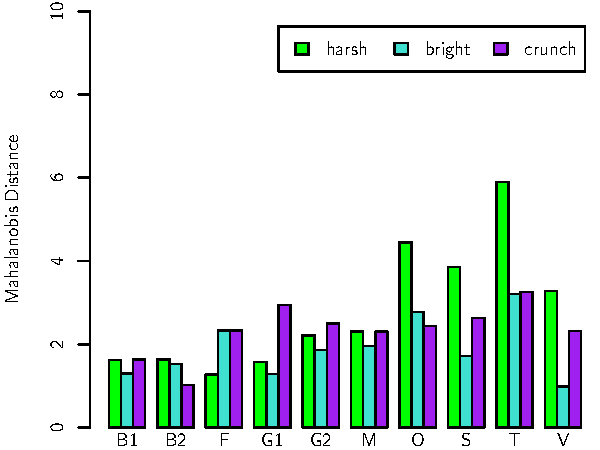
\includegraphics{chapter7/Images/CrunchProcessedJeffsDistance.pdf}
				\caption{Mahalanobis distances for the processed 
					 features of the harshness / crunchiness effect.}
				\label{tab:CrunchProcJeff}
			\end{figure}

			\begin{figure}[h!]
				\centering
				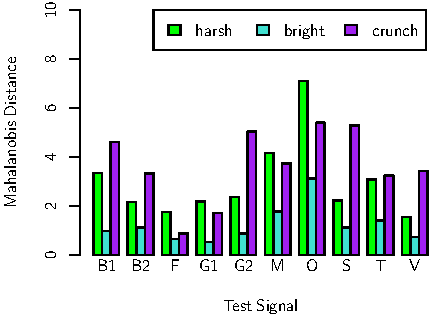
\includegraphics{chapter7/Images/CrunchDifferenceJeffsDistance.pdf}
				\caption{Mahalanobis distances for the feature differences of 
					 the harshness / crunchiness effect.}
				\label{tab:CrunchDiffJeff}
			\end{figure}

	\subsection{Evaluation Experiment}
	\label{sec:PerceptualExperiments-SemanticControl-EvaluationExperiment}
		\note{Randomised parameter slider and same order.}

	\subsection{Performance Results}
	\label{sec:PerceptualExperiments-SemanticControl-PerformanceResults}
		\note{Cophenetic distance.}

		\begin{figure}[h!]
			\centering
			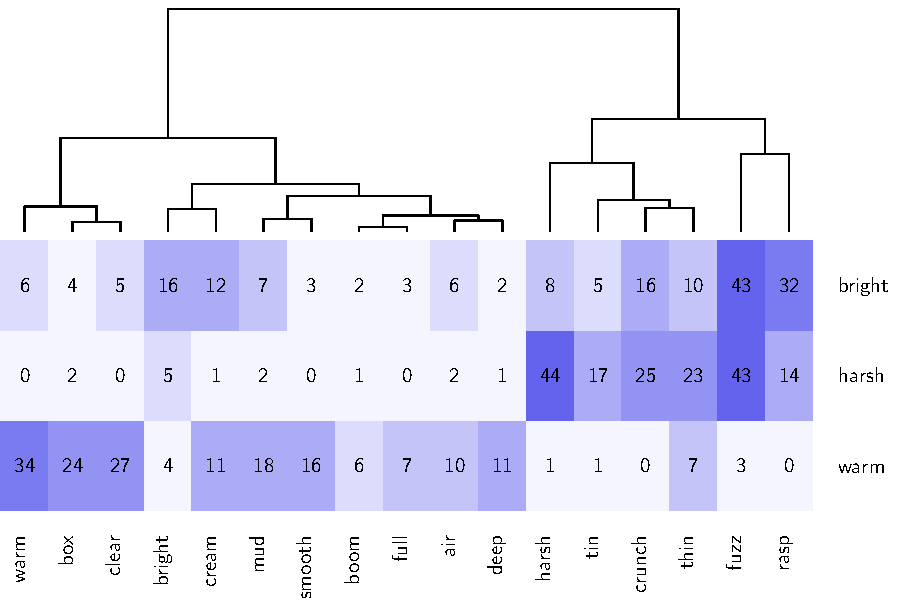
\includegraphics{chapter7/Images/HarshConfusion.pdf}
			\caption{Warmth / Harshness Confusion Matrix}
		\end{figure}

		\begin{figure}[h!]
			\centering
			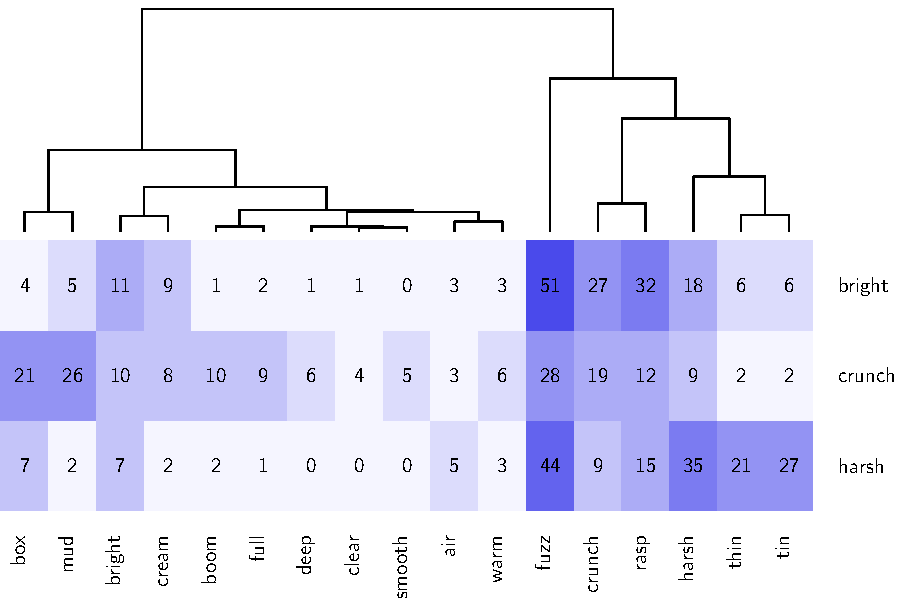
\includegraphics{chapter7/Images/CrunchConfusion.pdf}
			\caption{Harshness / Crunchiness Confusion Matrix}
		\end{figure}

		\begin{figure}[h!]
			\centering
			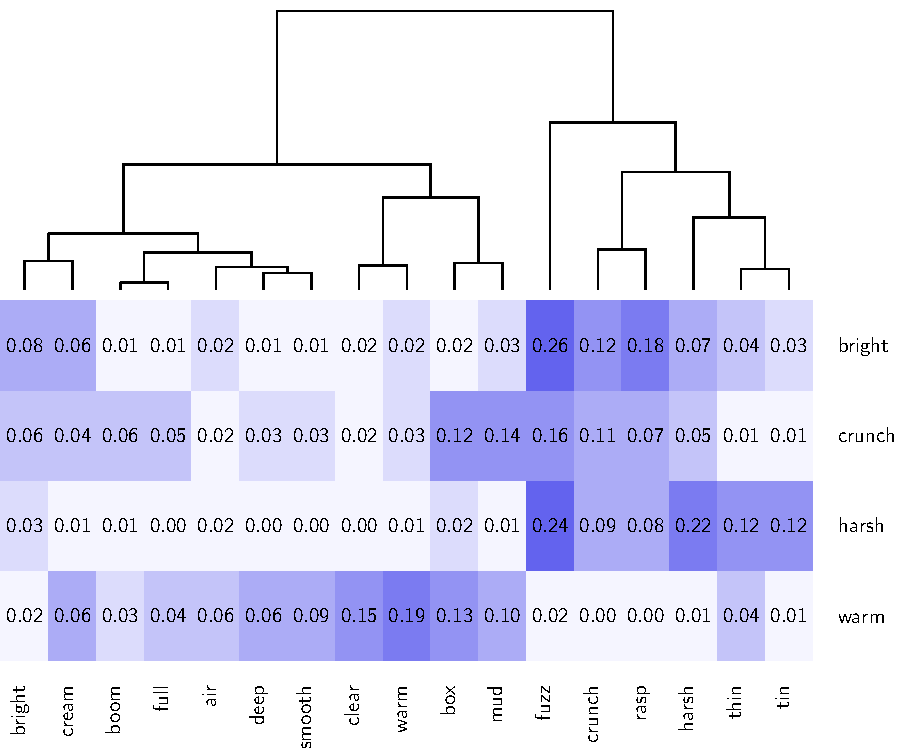
\includegraphics{chapter7/Images/CombinedConfusion.pdf}
			\caption{Combined Confusion Matrix}
		\end{figure}

		\begin{figure}[h!]
			\centering
			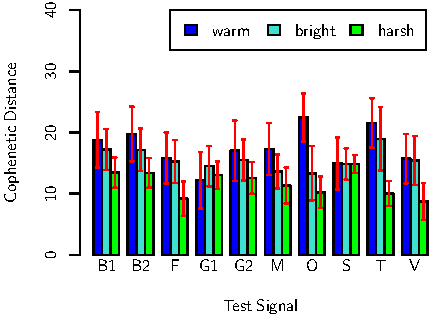
\includegraphics{chapter7/Images/HarshProcessedCophDistance.pdf}
			\caption{Harsh Processed}
		\end{figure}

		\begin{figure}[h!]
			\centering
			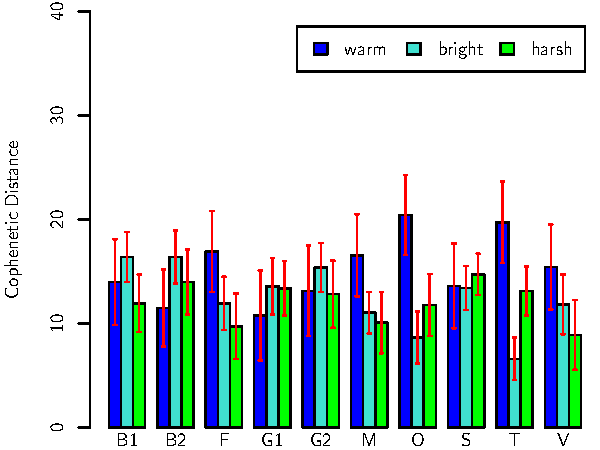
\includegraphics{chapter7/Images/HarshDifferenceCophDistance.pdf}
			\caption{Harsh Difference}
		\end{figure}

		\begin{figure}[h!]
			\centering
			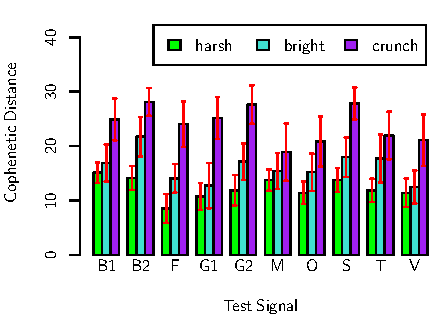
\includegraphics{chapter7/Images/CrunchProcessedCophDistance.pdf}
			\caption{Crunch Processed}
		\end{figure}

		\begin{figure}[h!]
			\centering
			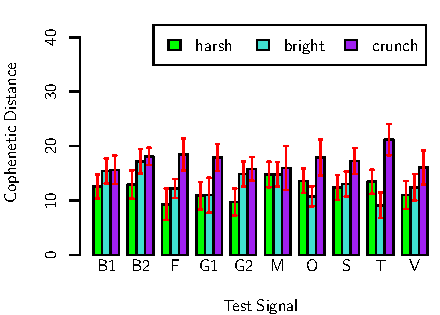
\includegraphics{chapter7/Images/CrunchDifferenceCophDistance.pdf}
			\caption{Crunch Difference}
		\end{figure}
